\clearpage
\vspace*{\fill}
\begin{figure}[H]
    \centering
      
\includegraphics[width=5cm]{src/cover/title_page_colorspace.png}%
\end{figure}
\vspace*{\fill}
\thispagestyle{empty}%
\clearpage

\chapter{developing a bit of a complex}
Psychedelia was just the beginning. 

\begin{definition}[Jeffrey Says]
\setlength{\intextsep}{0pt}%
\setlength{\columnsep}{3pt}%
\begin{wrapfigure}{l}{0.12\textwidth}

\includegraphics[width=\linewidth]{src/callout/psych.png} 
\end{wrapfigure}
\small
Colourspace is the second stage development of an idea which grew out of an
appreciation of good rock music, and an interest in the way in which music and
light go together.  Most people who attend rock concerts enjoy lighting effects
during the performance, often involving lasers and projections onto large
screens behind the group.  Such effects usually enhance the enjoyment of the
music for those watching.

What I wanted to do was make the lightshow playable in much the same way as a
musician plays his instrument.  An operator interpreting the music visually in
realtime could seriously blow the minds of people watching as well as having a
really good time himself.

The original idea was for a device to be played on stage and controlling large
lighting rigs and lasers, and obviously I had neither the cash or expertise to
build such a device, so it remained as only an idea until I decided to
experiment with using a computer to generate the effects on a TV screen, for
use in the home.
\end{definition}

\clearpage
\begin{figure}[H]
    \centering
    \begin{adjustbox}{width=12cm,center}
    \frame{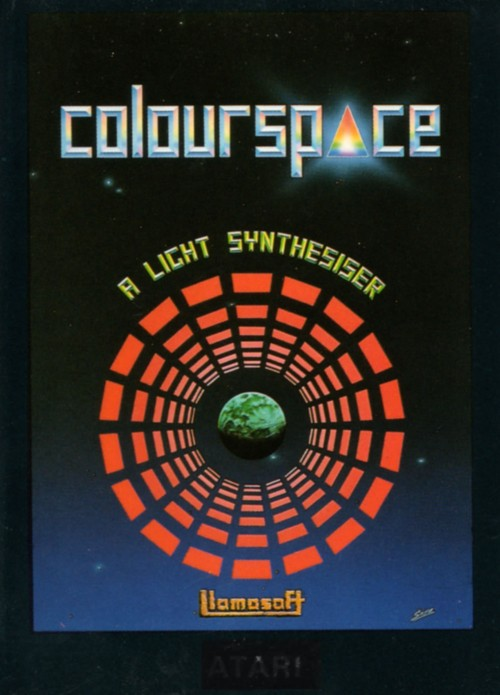
\includegraphics{src/preface_colorspace/colorspace.jpg}}%
    \end{adjustbox}
\caption{Cover art by Steinar Lund for the commercial edition of Colourspace}
\end{figure}
\clearpage
\begin{definition}[Jeffrey Says]
\setlength{\intextsep}{0pt}%
\setlength{\columnsep}{3pt}%
\begin{wrapfigure}{l}{0.12\textwidth}

\includegraphics[width=\linewidth]{src/callout/psych.png} 
\end{wrapfigure}
\small
The resultant program, PSYCHEDELIA, is now available for many popular micros,
and has freaked quite a few people out.  Using keyboard and joystick, operators
can produce lightshows to accompany their favourite music.  The displays have
been described as being like "interactive fireworks".  Whilst satisfying on
their own, the displays are best to the accompanyment of loud music, which acts
like a catalyst and vastly increases the enjoyment of playing.  The system is
set up like a synthesizer, with user-controllable variables defining the modes
of pattern-generation.  Users "perform" using the joystick and can store away
effects for later recall by a single keypress.
This program, COLOURSPACE, is based upon the same basic idea.  By using the
unique Atari screen hardware and colour pallette, the effect of the program is
much improved.  The difference between Psychedelia and Colourspace is as
pronounced as the difference between a Mini and a Ferrari.  Using the Atari you
can get curved screens, hardware reflections, interlace effects, stroboscopics,
dynamic colourflows, and variable resolution screens.  There are 80 presets
available for programming, 16 user-definable lightforms, and a foreground
drawing mode.  There is even a mode which allows you to perform simultaneously
with another player or with the computer.
\end{definition}


